\documentclass[12pt]{article}
\usepackage{geometry} % Pour passer au format A4
\geometry{hmargin=1cm, vmargin=1cm} % 

% Page et encodage
\usepackage[T1]{fontenc} % Use 8-bit encoding that has 256 glyphs
\usepackage[english,french]{babel} % Français et anglais
\usepackage[utf8]{inputenc} 

\usepackage{lmodern}
\setlength\parindent{0pt}

% Graphiques
\usepackage{graphicx,float,grffile}
\usepackage{pst-eucl, pst-plot} 

% Maths et divers
\usepackage{amsmath,amsfonts,amssymb,amsthm,verbatim}
\usepackage{multicol,enumitem,url,eurosym,gensymb}

% Sections
\usepackage{sectsty} % Allows customizing section commands
\allsectionsfont{\centering \normalfont\scshape}

% Tête et pied de page

\usepackage{fancyhdr} 
\pagestyle{fancyplain} 

\fancyhead{} % No page header
\fancyfoot{}

\renewcommand{\headrulewidth}{0pt} % Remove header underlines
\renewcommand{\footrulewidth}{0pt} % Remove footer underlines

\newcommand{\horrule}[1]{\rule{\linewidth}{#1}} % Create horizontal rule command with 1 argument of height

%----------------------------------------------------------------------------------------
%	Début du document
%----------------------------------------------------------------------------------------

\begin{document}

%----------------------------------------------------------------------------------------
% RE-DEFINITION
%----------------------------------------------------------------------------------------
% MATHS
%-----------

\newtheorem{Definition}{Définition}
\newtheorem{Theorem}{Théorème}
\newtheorem{Proposition}{Propriété}

% MATHS
%-----------
\renewcommand{\labelitemi}{$\bullet$}
\renewcommand{\labelitemii}{$\circ$}
%----------------------------------------------------------------------------------------
%	Titre
%----------------------------------------------------------------------------------------

\setlength{\columnseprule}{1pt}

\section*{ie - Théorème de Thalès}
\begin{center}
  \textit{Théophraste- La plus coûteuse des dépenses, c’est la perte de temps.}
\end{center}
\horrule{2px}

\subsection*{ex1 - Calculer}
\textit{Trouver le nombre à l'aide du produit en croix. Écrire le calcul et donner la réponse.}

\begin{multicols}{4}

  \begin{center}
    \begin{tabular}{|c|c|}
      \hline
      12 & 8  \\
      \hline 
      & 2  \\
      \hline
    \end{tabular}

    \begin{tabular}{|c|c|}
      \hline
      10 & 9  \\
      \hline 
      24 &   \\
      \hline
    \end{tabular}

    \begin{tabular}{|c|c|}
      \hline
      7 &   \\
      \hline 
      45  & 21  \\
      \hline
    \end{tabular}

    \begin{tabular}{|c|c|}
      \hline
      & 12,4  \\
      \hline 
      9,2  & 3,6  \\
      \hline
    \end{tabular}
  \end{center}
\end{multicols}

\subsection*{ex2 - Modéliser}
\textit{Il faut rédiger rigoureuseuement, sans oublier les étapes.}

\begin{multicols}{2}

  \subsection*{2.1}

  \begin{multicols}{2}

    Les droites (JR) et (DH) sont parallèles.\\
    On donne QR = 5,7 cm, QD = 3,6 cm, DH = 5 cm et HR = 2,8 cm.\\
    \textbf{Calculer QJ et JR.}
    \begin{figure}[H]
      \centering
      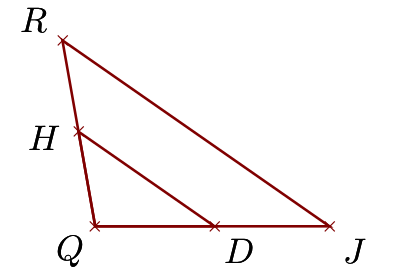
\includegraphics[width=.5\linewidth]{4x6-thales/sources/th1.png}
    \end{figure}

  \end{multicols}

  \subsection*{2.2}
  \begin{multicols}{2}
    Les droites (PR) et (WS) sont parallèles.\\
    On donne EP = 5,9 cm, ER = 4,6 cm, W S = 1,4 cm et SR = 6,7 cm.\\
    \textbf{Calculer PR et EW.}
    \begin{figure}[H]
      \centering
      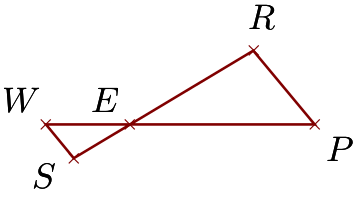
\includegraphics[width=.5\linewidth]{4x6-thales/sources/th2.png}
    \end{figure}
  \end{multicols}


  \subsection*{2.3}
  \begin{multicols}{2}
    Les droites (PL) et (CW) sont parallèles.\\
    On donne OL = 6 cm, PL = 5,1 cm, OC = 2,1 cm et WL = 2,9 cm.\\
    \textbf{Calculer OP et CW.}
    \begin{figure}[H]
      \centering
      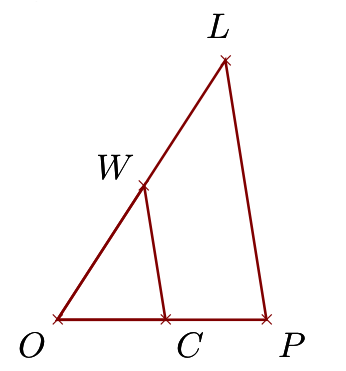
\includegraphics[width=.5\linewidth]{4x6-thales/sources/th3.png}
    \end{figure}
  \end{multicols}


  \subsection*{2.4}
  \begin{multicols}{2}
    Les droites (CP ) et (LS) sont parallèles.\\
    On donne MC = 1,5 cm, MP = 1,7 cm, CP = 1,6 cm et LS = 0,5 cm.\\
    \textbf{Calculer ML et MS.}
    \begin{figure}[H]
      \centering
      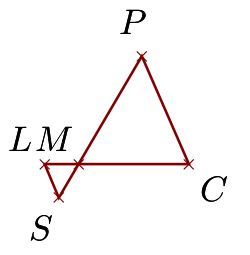
\includegraphics[width=.5\linewidth]{4x6-thales/sources/th4.png}
    \end{figure}
  \end{multicols}
\end{multicols}

\begin{multicols}{3}
  \subsection*{ex3 - Raisonner}
  Pour consolider un bâtiment, on a construit un contrefort en bois. \\
  Sur le dessin, on donne : BS = 6 m ; BN = 1,8 m ; AS = 6,5m ; AB = 2,5m.\\
  \textbf{Calculer MN, SM et AM.}
  \begin{figure}[H]
    \centering
    \includegraphics[width=.5\linewidth]{4x6-thales/sources/mur.pdf}
  \end{figure}


  \subsection*{ex4 - Representer}
  Lilia souhaite préparer un spectacle de marionnettes en ombres chinoises. \\
  Son écran mesure 2m de haut. Il est aligné à sa marionnette qui mesure 24cm.
  Elle tient sa marionnette à 30 cm de la lumière.\\
  A quelle distance de la lumière doit-elle placer l’écran pour agrandir sa marionnette au maximum ?

  \textbf{Représenter la situation sur un schéma.}
\end{multicols}


\end{document}
